\documentclass[a4paper,12pt]{article}
\usepackage{amsfonts}
\usepackage{amssymb}
\usepackage{latexsym}
\usepackage{amsmath}
\usepackage{amsthm}
\usepackage{float}
\usepackage{graphicx}
\usepackage{indentfirst}
\usepackage[polish]{babel}
\usepackage[T1]{fontenc}
\usepackage[utf8]{inputenc}
\usepackage{wrapfig}
\usepackage{setspace}
\usepackage{array}
\usepackage{multirow}
\usepackage{geometry}
\usepackage{subfig}
\geometry{hdivide={2cm,*,2cm}}
\geometry{vdivide={2cm,*,2cm}}
\usepackage{titlesec}
\titlespacing{\section}{0ex}{1ex}{1ex} % zmniejszenie odstêpów przed i po tytule rozdzia³u...
\titleformat*{\section}{\sf\large\bfseries} % i zmiana kroju czcionki
\titlespacing{\subsection}{0ex}{0.75ex}{0.75ex} % % j/w dla tytu³ów podrozdzia³ów
\titleformat*{\subsection}{\sf\bfseries}

% Zmniejszenie odstêpów przed i za wzorami wystawionymi
\AtBeginDocument{
\addtolength{\abovedisplayskip}{-1ex}
\addtolength{\abovedisplayshortskip}{-1ex}
\addtolength{\belowdisplayskip}{-1ex}
\addtolength{\belowdisplayshortskip}{-1ex}
}
% Kilka przydatnych definicji
\newcolumntype{C}[1]{>{\centering\arraybackslash}m{#1}}
\newcommand{\razy}{\hspace{-0.5ex}\times\hspace{-0.5ex}} % mo¿e siê przydaæ

\begin{document}
\def\tablename{Tabela} % bez tej linii nazw¹ tabeli by³aby "Tablica"
\noindent
\textbf{Sebastian Prokop, 320728, grupa 4, projekt 2, zadanie 35}

%%% Nie do końca rozumiem wszystko co się dzieje powyżej. Poniżej jest część, którą ja zrobiłem 

\section*{Wstęp}
Metodą potęgową z normowaniem można - przy spełnieniu odpowiednich warunków - wyznaczyć dominującą wartość własną macierzy. Przy dodaniu do tego deflacji, w tym projekcie realizowanej za pomocą obrotów Givensa, można znaleźć ich więcej. Metoda potęgowa jest iteracyjna, dlatego można żądane efekty osiągnąć z różną dokładnością i w różnym czasie. Wynik jej działania jest zależny również od samych wartości własnych badanej macierzy. Okazuje się ona być skuteczna i dokładna przy spełnieniu warunkó zbieżności.

\section*{Opis matematyczny}
Pierwszym krokiem jest wyznaczenie wektora własnego odpowiadającego wartości własnej z największym modułem. W tym celu powtarza się następujące operacje:
\[ \widetilde{x}^{(k)} = \frac{x^{(k)}}{\lVert x^{(k)} \rVert} \;\;\; , \;\; x^{(k+1)} = A\widetilde{x}^{(k)} \;\;\; , \;\; (k = 0,1...), \]
gdzie $x$ jest wyznaczanym przybliżeniem wektora własnego, natomiast $A$ jest macierzą, której wartości własnych szukamy. Warunek stopu jest następujący:
\[ |sign(\widetilde{x}_i^{(k+1)}) \cdot \widetilde{x}^{(k+1)} - sign(\widetilde{x}_i^{(k)}) \cdot \widetilde{x}^{(k)}|<d,\]
gdzie $d$ jest parametrem określającym dokładność, a $\widetilde{x}_i^{(k)} = max_{1\leq j\leq n}|\widetilde{x}_j^{(k)}|$, czyli jest elementem o największym module. Warunki zbieżności to posiadanie dominującej wartości własnej, dlatego oprócz sprawdzania powyższej nierówności, istnieje drugi warunek zakończenia - osiągnięcie maksymalnej ilości iteracji. Wektor $x^{(0)}$ musi być taki, że w jego zapisie jako kombinacji liniowej wektorów własnych, współczynnik przy wektorze własnym odpowiadającym dominującej wartości własnej jest niezerowy. Jest on więc brany jako losowy, ponieważ wtedy szansa na niespełnienie tego warunku jest pomijalnie mała.

\section*{Eksperymenty Numeryczne}
Wyniki działania dla macierzy o wartościach własnych ${6, -5, 3}$ dla różnych dokładności i maksymalnej ilości iteracji równej $3\cdot 10^6$ przedstawia tabela 1.
\begin{table}[h!]
    \centering
\begin{tabular}{|l|l|l|l|}
\hline
$\lambda_1 = 6$                & $\lambda_2 = -5$                 & $\lambda_3 = 3$                 & d      \\
\hline
3.941734806360585          &    2.175293847303345           & -2.117028653663931           & 1      \\
\hline
5.990891457126361            &   -4.993840444390946           &    3.002948987264586           & 1e-2    \\
\hline
6.000000919054853 & -5.000000606448076 & 2.999999687393222 & 1e-6    \\
\hline
6.000000000000001 & -5.000000000000001 & 3.000000000000001 & 1e-15  
\\
\hline
\end{tabular}
    \caption{Wyniki dla prostej macierzy i różnych wartości parametru d}
    \label{tab:my_label}
\end{table}
Można zauważyć, w szczególności przy bardzo niskiej wymaganej dokładności, że wyniki różnią się przy kolejnych wywołaniach \emph{test1}. Wynika to z faktu, że początkowy wektor przybliżeń jest losowy i inny w każdym wywołaniu programu. 

W powyższym przykładzie macierz miała wartości własne o różnych modułach. W przeciwnym przypadku badana metoda nie gwarantuje otrzymania wyniku, ponieważ nie jest spełniony warunek zbieżności. Okazuje się jednak, że przy mało restrykcyjnej tolerancji na błąd, można uzyskać przybliżenia wartości własnych również w takich przypadkach. Pokazuje to tabela 2.

\begin{table}[H]
    \centering
\begin{tabular}{|l|l|l|l|}
\hline
$\lambda_1 = 3$                & $\lambda_2 = 1$                 & $\lambda_3 = -1$                 & d      \\
\hline
3.000193349723464 & 0.995158536018855 & -0.995351885742319 & 1e-3 \\
\hline
3.000060239943521 & 1.000464958096908 & -1.000525198040429 & 1e-4 \\
\hline
2.999998709039096 & brak              & brak               & 1e-5 \\
\hline
2.999999196693963 & brak              & brak               & 1e-6 \\
\hline
\end{tabular}
    \caption{Wyniki dla macierzy z ww. 3, 1, -1, $iter = 3e6$}
    \label{tab:my_label2}
\end{table}
\vspace{-6mm}%Put here to reduce too much white space after your table
Sytuacja wygląda inaczej, gdy istnieją dwie takie same wartości własne o największym module. Wtedy w poniższym przykładzie udało się je policzyć z dużą dokłądnością. Przedstawia to tabela 3. 

\begin{table}[H]
    \centering
\begin{tabular}{|l|l|l|l|}
\hline
$\lambda_1 = 5$                & $\lambda_2 = 5$                 & $\lambda_3 = 0$                 & d      \\
\hline
5.000003021401001 & 4.999996978598999 & 0.000000000000000 & 1e-12 \\
\hline
brak              & brak              & brak              & 1e-13 \\
\hline
\end{tabular}
   \footnotesize \caption{Wyniki dla macierzy z ww. 5, 5, 0, $iter = 3e6$}
    \label{tab:my_label3}
\end{table}
\vspace{-6mm}%Put here to reduce too much white space after your table
Jednocześnie można jednak zauważyć, że o ile w tabeli 1 istniała wyraźna korelacja między parametrem \emph{prec} a liczbą cyfr po przecinku które pasowały do poprawnego wyniku, tak tym razem mimo, że \emph{prec} jest ustawiony na 1e-12, wyniki pokrywają się jedynie do piątego miejsca po przecinku.

\section*{Błąd teoretyczny a rzeczywisty}
Zgodnie z teorią, w badanej metodzie, błąd maleje tak szybko jak wyrażenie
\[ s =|\lambda_1^{-1} \cdot \lambda_2|^k ,\]
gdzie $\lambda_1$ i $\lambda_2$ to dwie największe co do modułu wartości własne. W \emph{test4} badana jest macierz, której $ \lambda_1  = 6$ i $\lambda_2 = -5$. Test przedstawia na wykresie kolejne wartości przybliżenia $x^{(k)}$ i przebiegu wartości wyrażenia $s(k)$. Wyniki uzyskane dla dwóch różnych przybliżeń początkowych przedstawiają Rysunek 1a i 1b.
\begin{figure}[H]%
    \centering
    \subfloat[\centering Dla $x^{(0)}$ będącego wektorem jedynek.]{{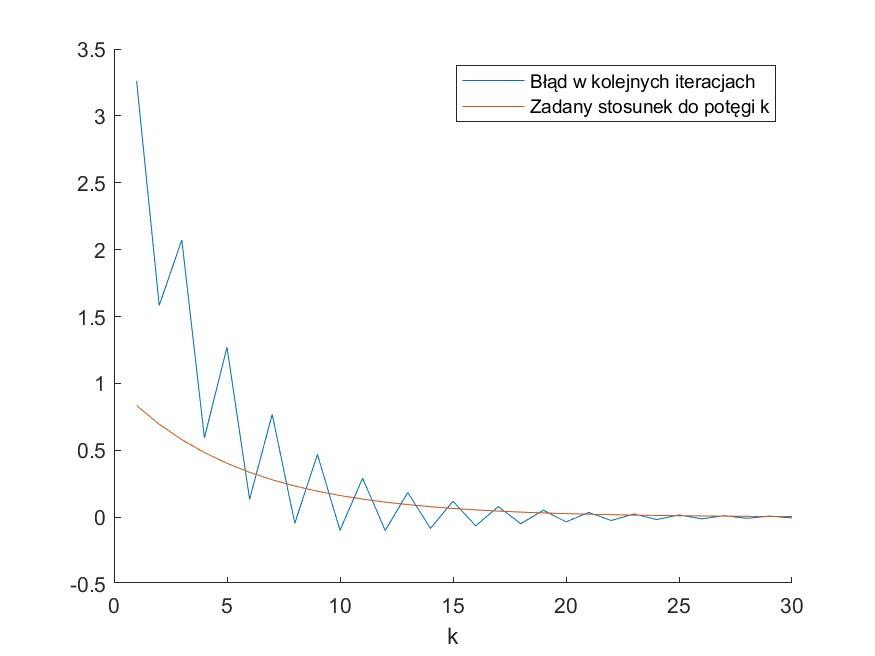
\includegraphics[width=7.5cm]{fig1.jpg} }}%
    \qquad
    \subfloat[\centering  Dla $x^{(0)}$ będącego wektorem losowym.]{{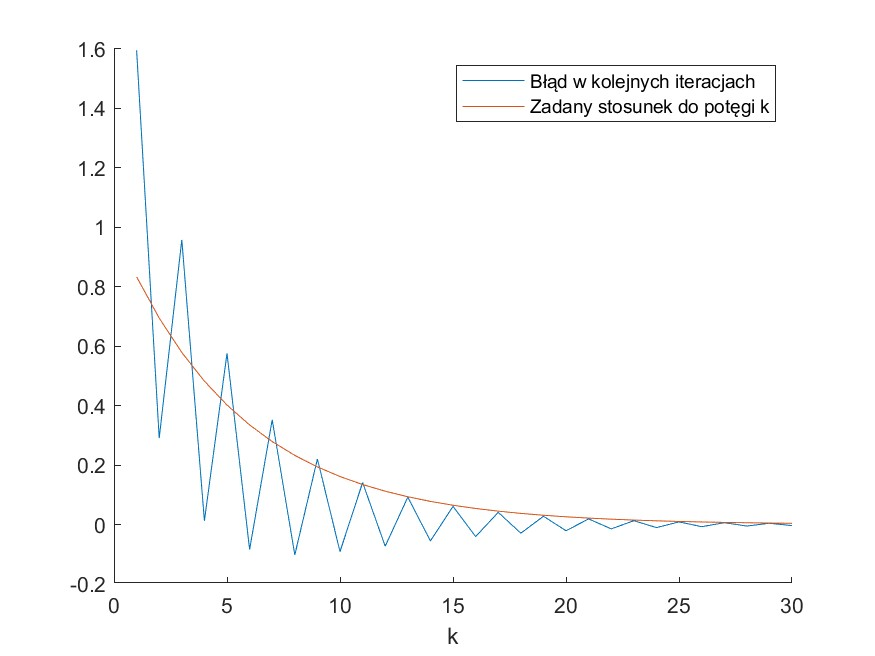
\includegraphics[width=7.5cm]{fig2.jpg} }}%
  \footnotesize \caption{Wykresy błędu przybliżenia wartości własnej } %
    \label{fig:example}%
\end{figure}
\vspace{-6mm}%Put here to reduce too much white space after your table
Warto uruchomić \emph{test4} kilka razy, żeby zaobserwować różnice - wektor początkowy jest za każdym razem inny.

\section*{Podsumowanie}
Metoda potęgowa z normowaniem okazuje się być skuteczna, czasem wyznaczając poprawne wartości bez spełnionych warunków zbieżności. Wpływ na wynik ma również losowy początowy wektor przybliżenia, który ma wpływ na to w ilu iteracjach zostanie osiągnięta żądana dokładność.


\end{document}